\chapter{Cluster labeling}
A major problem in text analysis is to determine the topics in a text collection and identify the most important or significant relationships between them. Clustering and visualization (e.g. in the form of tag clouds) are key analysis methods in order to address this problem. In this chapter, an algorithm for cluster labeling, which is relatively new, is discussed, and in Chapter~\ref{sec:tagclouds} tag clouds are introduced as a visualization mean used in \gls{IR} systems. \\

\section{Clustering}
\textit{Clustering} is an \gls{IR} method that groups objects (documents) together based on their similarities in so called clusters. Such methods are often applied in the post processing phase of \gls{IR}~(fig.~\ref{fig:text_analysis}) for the visualization of retrieved results. For example, similar search results can be grouped together during presentation of results in search engines. \\

Clustering can be used to categorize resources. \textit{Document categorization} is the process of assigning a document to one or more categories. A categorization $C = \{c_{1}, c_{2}, ..., c_{k}\}$ partitions a document collection $D$ into subsets $c \subseteq D$, so that $ \cup_{i=1}^{k} c_{k} =D $. $C$ is an exclusive categorization if $c_{i} \cap c_{j \ne i} = 0, c_{i}, c_{j} \in C$, and non-exclusive categorization otherwise. Clustering is an \textit{unsupervised categorization method}, as it organizes documents into clusters without having prior knowledge about the clusters, or predefined cluster categories.\\
 

Presenting search results in groups, or categories, should help users gain a quick overview of the retrieved documents. An important part of clustering used for visualization of results, is to choose suitable labels of the categories defined, so that they are usable to human users. The process of \textit{cluster labeling} automatically creates labels for clustered groups of objects. \\

\subsection{Clustering algorithms}
\label{sec:clustering_algorithms}
A large variety of clustering algorithms exists, and they are usually classified according to the characteristic of their output structure. Jain et al.~\cite{clusteringJain99} make a classification based on the following properties: \\

\textbf{Flat vs. hierarchical clustering} \\
\textit{Flat clustering} creates a flat set of clusters without relations between clusters due to some structure. K-means is a popular clustering algorithm, which creates as output a flat structure of document clusters. The k-means clustering algorithm is presented as an example for flat clustering in section~\ref{clustering:algo}. \textit{Hierarchical clustering} on the other hand creates a hierarchy of clusters, with parents and children nodes, in a tree-like manner~(Johnson~\cite{hierarchical_clustering}). \\

\textbf{Hard vs. soft clustering}\\
Another important distinction can be made between \textit{hard} and \textit{soft} (also called fuzzy) clustering algorithms. If each document is assigned to a single cluster only, we have hard clustering. Otherwise, clustering is soft, and it assigns a document as a distribution over all clusters. This means that each document can have a fractional membership in several clusters. \gls{LSA}~(Chapter~\ref{sec:lsa}) is a good example for a soft clustering algorithm. K-means is a popular example for hard clustering~(section~\ref{clustering:algo}). \\


\textbf{Monothetic vs. polythetic clustering} \\
Based on how documents are assigned to different clusters, clustering can be divided into \textit{monothetic} and \textit{polythetic}~\cite{hierarchMonotheticClustering2004}. Monothetic algorithms assign a document to a cluster based on a single feature, while polythetic algorithms classify documents by overall degree of similarity/difference calculated over many properties. This makes monothetic clustering well suited for generating hierarchies and browsing search results, since a single feature, common to all documents in the cluster, describe each cluster. Users understand easily clusters generated in this way. K-means is an example of polythetic document clustering algorithm, where each cluster is described by several words of phases. \\



\subsection{K-means clustering algorithm}
\label{clustering:algo}
In this work the cluster labeling algorithm Weighted Centroid Covering is evaluated. As clustering precedes cluster labeling, the k-means algorithm is used for document clustering. Two factors influence this implementation decision:
\begin{itemize}
\item As \gls{LSA} is used to process the term-document matrix, it can be investigated which dimensionality reduction parameter $k$ is optimal for the specific implementation in this work, so that the optimal number of topics (or soft clusters) can be obtained for the evaluation data set. Therefore, the dimensionality reduction parameter, previously defined in \gls{LSA}, can be used as initial parameter for k-means, or the number of clusters inputed to the algorithm. Thus, one of k-means' weaknesses will not affect this work. 
\item Another reason to use k-means algorithm is its simplicity, as compared for example to \gls{HAC} - the complexity of k-means is linear, while the complexity of \gls{HAC} is exponential. \\
\end{itemize}

\textit{K-means} is an example for a flat, hard and polythetic clustering algorithm, based on the classification mentioned previously. It was first introduced by Lloyd~\cite{kmeans_Lloyd82}. The algorithm outputs a flat unstructured set of clusters. It starts by dividing the document collection into $k$ clusters, where $k$ is an input parameter, and then computes the $k$ \textit{means} of these clusters. K-means defines a cluster in terms of a \textit{centroid}, usually the \textit{mean of a group of points}, and is applied to objects (documents) in n-dimensional space (such as vector space). After the initialization, the following two steps are iteratively repeated, until the clusters are not re-assigned any more: \\
\begin{enumerate}
\item Each document in the collection is assigned to the cluster with the closest mean.
\item For each cluster, new means are recomputed based on the documents it contains.
\end{enumerate}

In algorithm~\ref{algorithm_kmeans}a detailed step-by-step description of the k-means algorithm is given as pseudo-code. \\


\renewcommand{\algorithmicrequire}{\textbf{Input:}}
\renewcommand{\algorithmicensure}{\textbf{Output:}}
\begin{algorithm}
\caption{K-means clustering algorithm}
\label{algorithm_kmeans}
\begin{algorithmic}
\REQUIRE $D = \{d_{1}, d_{2}, ..., d_{n}\}$ - documents to be clustered \\
         $k$ - number of clusters \\
\ENSURE $C = \{c_{1}, c_{2}, ..., c_{k} \}$ - clusters \\
        $ m : D \rightarrow \{1 ... k \} $ - cluster membership \\
\STATE Set $C$ to initial value (e.g. select $k$ random points as initial centroids) \\
\COMMENT{Form $k$ clusters by assigning each document to its closest centroid}
\FORALL{$d_{i} \in D$}
\STATE $m(d_{i}) = mindistance_{j \in \{1..n \}}(d_{i}, c_{j})$
\ENDFOR \\
\COMMENT{Recompute the centroid of each cluster until centroids do not change}\\
\WHILE{$m$ has changed}
\FORALL{$ i \in \{1..n \}$}
\STATE Recompute $c_{i}$ as the centroid of $ \{d | m(d) = i \} $
\ENDFOR
\FORALL{$d_{i} \in D$}
\STATE $m(d_{i}) = mindistance_{j \in \{1..n \}}(d_{i}, c_{j})$
\ENDFOR
\ENDWHILE
\end{algorithmic}
\end{algorithm}

\textbf{TODO}: Give + and - of this method. \\

\section{Cluster labeling}
\label{sec:cluster_labeling}
Assume that a categorization over a document collection is determined using an unsupervised approach, such as clustering. To present this categorization to users, it is convenient to label the individual categories with characteristic terms. These terms, called \textit{category labels}, should characterize the content of the associated category with respect to the remaining categories. This implies that cluster labeling should \textit{summarize} a category's content and that it should \textit{discriminate} a category from the remaining categories. This section states desired properties for category labels and presents the Weighted Centroid Covering algorithm~(Stein and Meyer zu Eissen~\cite{Stein04topicidentification}) which generates such labels. It further makes a proposition for improvement of \gls{WCC}~(section~\ref{clustering:WCC}). Finally, in Chapter~\ref{sec:implementation} an evaluation of \gls{WCC} for labeling document clusters is offered, created using k-means algorithm. \\

\subsection{Clustering and labeling}
In their paper from 2009~\cite{surveyWebClusteringEngines2009}, Carpineto et al. claimed that there is a difference between clustering of data sets, and clustering of search results, returned from search engines:~\textit{"in search results clustering description comes first"}. Thus, in contrast to the classical categorization of clustering algorithms previously outlined, they proposed a classification based on how well the clustering algorithms can generate sensible, comprehensive and compact cluster labels, and divided the algorithms in the following three categories: \\

\textbf{Data-centric algorithms} \\
Data-centric algorithms were the first ones to be implemented for cluster labeling. Here, clustering is done with some general clustering algorithm, and terms which are close to the cluster centroids are nominated as cluster labels. Cluster centroids are a collection of independent terms from all documents not related to each other. In order to define the terms from cluster centroid, one uses a frequency measure, such as $tf-idf$~(eq.~\ref{lsa:tf_idf}). \gls{WCC}~(see~\ref{clustering:WCC}) is presented as an example for a data-centric clustering algorithm. \\

\textbf{Description-aware algorithms} \\
While data-centric algorithms don't consider word order, and process documents as "a bag of words", description-aware algorithms process ordered sequence of words (phrases), instead of terms, as candidate labels, and assign labels during clustering process, not after it. Using monothetic term selection, one nominates frequent phrases containing a noun head as labels, which are interpretable to human users. Clustering and labeling are closely related, and labeling influences the clustering process. Therefore, it is not possible to combine the labeling with any clustering algorithm. \gls{STC} is an example of a description-aware algorithm, introduced by Zamir and Etzioni~\cite{suffixTreeClustering99}. \gls{STC} builds a tree from the most frequent phrases in documents by using the data structure \textit{suffix tree}~\cite{suffixTreeClustering99}. It group documents that have common phrases under the same nodes of the tree. Thus, all documents below a given node contain the phrase at the node. \\

\textbf{Description-centric algorithms} \\
These algorithms operate on the principle \textit{"description comes first"}, and in this sense are the opposite of the data-centric algorithms. The goal here is to find meaningful cluster labels. If there are no suitable labels found, the cluster has no value for the users (doesn't have a proper visualization), and is therefore discarded. Description-centric algorithms are mainly applied for clustering of search results~(more information can be found in~\cite{surveyWebClusteringEngines2009}). \\

\subsection{Formal framework for cluster labeling algorithms}
When an unsupervised approach is used to categorize a collection of documents, such as clustering, it is also necessary to label the categories defined, in order to present them to users. The category labels should characterize the given categories - labels should summarize category content, and should discriminate a category from other categories~\cite{Stein04topicidentification}. Until now, no uniformly agreed upon formal framework exists that defines the requirements for cluster labeling algorithms. There are publications which name desired properties for cluster labels (\cite{formal_cluster_labels2003},~\cite{dweiss2006} ), but they all give informal descriptions. Stein and Meyer Zu Eissen~\cite{Stein04topicidentification} have given their definitions for desired properties of cluster labeling algorithms as a formal framework. The definition presented below is based on this source. \\

If we have an unstructured collection of documents $D$, a clustering algorithm creates a categorization for this collection in the form $ C = \{ c_{1}, c_{2}, ..., c_{k} \} $, where the sets $c_{i}$ are subsets of $D$, and their union covers $D$: $\cup_{c_{i}\in C} c_{i} = D$. When applying a hierarchical clustering algorithm, this implies a cluster labeling hierarchy $H_{C}$ over $C$. Then, $H_{C}$ is a tree and its nodes are the categories in $C$, having one node as a root. Let $c_{i}, c_{j} \in C, c_{i} \ne c_{j}$ are two categories. If $c_{j}$ is a child cluster of $c_{i}$, then $c_{i}$ is closer to the root of the hierarchy $H_{C}$, and we write $c_{i} \succ c_{j}$. \\

For an existing categorization $C$, we therefore need a cluster labeling $ \text{\L} = \{ l_{1}, l_{2}, ..., l_{k} \} $. \\


Let $T = \cup_{d \in D}T_{d} $ be the term set in the given document collection $D$. As defined by Stein and Meyer zu Eissen~\cite{Stein04topicidentification}, a cluster labeling function $ \tau : c \shortrightarrow \text{\L} $ assigns a cluster label to each cluster $ c \in C $, where $\text{\L}_{c} \subset T$. \\


Thus, the following properties are desired for a cluster labeling function: \\
\begin{enumerate}
\item \textbf{Unique} \\
Cluster labels should be unique. The same terms should not be assigned as cluster labels to more than one cluster, or no two labels should include the same terms from two different clusters. \\
\begin{equation}
\forall_{
\substack{ c_{i},c_{j} \in C, \\ c_{i}\neq c_{j}}
} : \tau(C_{i}) \cap \tau(C_{j}) = 0
\end{equation}

 
\item \textbf{Summarizing} \\
If possible, the label of a cluster $c$ should contain at least one term $t$ from each document $ d\in c$. Terms occurring in all documents, which are part of the cluster, represent it better than terms that occur only in few documents. \\
\begin{equation}
\forall_{ c \in C}, \forall_{ d \in c} : \tau{c} \cap T_{d} \neq 0
\end{equation}
where $T_{d}$ is the set of terms in document $d$.

\item \textbf{Discriminating} \\
Apart from summarizing, terms in labels should be discriminating. They should contribute to discriminate the cluster from other clusters, i.e. the same terms should be present in a considerably smaller set of documents in the other clusters. In cluster label $c$ exists a term $t$ whose frequency of occurrence is relatively higher in the documents of the cluster as compared to other clusters. \\
\begin{equation}
\forall_{
\substack{ c_{i},c_{j} \in C \\ c_{i}\neq c_{j}}}
 \exists_{ t \in T{c_{i}}} : \frac{tf_{c_{i}}(t)}{\left| c_{i} \right|} \ll \frac{tf_{c_{i}}(t)}{\left| c_{j} \right|}
\end{equation}
Here, $T_{c_{i}}$ is the term set in category $c_{i}$, and $tf_{c_{i}} (t)$ is the term frequency of term $t$ in category $c_{i}$, or the sum of $tf (t)$ in all documents in cluster $c_{i}$ : $tf_{c_{i}} (t) = \sum_{d \in c_{i}}{tf_{d} (t)} $. \\


\item \textbf{Expressive} \\
Terms forming a label of cluster $c$ should have highest frequency of occurrence in the documents from $c$:
\begin{equation}
\forall_{c \in C} \forall_{d \in c} \forall_{t \in T_{d}} : tf_{d}(t) \leq tf_{d}(t'), t' \in \tau(c)
\end{equation}
Here, $tf_{d}(t)$ is the term frequency of occurrence of term $t$ in document $d$.

\item \textbf{Contiguous} \\
This property holds for consecutive terms, for example belonging to a phrase. Such cluster labels, containing consecutive terms, are more understandable to human users.
\begin{equation}
\forall_{c \in C} \forall_{
\substack{t, t' \in \tau(c), \\ c_{i} \ne c_{j}}
} \forall_{d \in c} \exists_{t_{i}, t_{i+1} \in T_{d}} : t_{i} = t \wedge t_{i+1} = t'
\end{equation}

\item \textbf{Hierarchically consistent}
\begin{equation}
\forall_{
\substack {c_{i}, c_{j} \in C, \\ c_{i} \ne c_{j}}
} : c_{i} \succ c_{j} \Rightarrow P(t_{i} | t_{j}) = 1 \wedge P(t_{j} | t_{i}) < 1,
\end{equation}
where $t_{i} \in \tau(c_{i})$ and $ t_{j} \in \tau(c_{j}) $. This property is required only when using a hierarchical clustering algorithm (e.g. \gls{STC}~\cite{suffixTreeClustering99}).

\item \textbf{Irredundant} \\
Irredundancy complements the property \textit{unique}. Terms which are synonyms should be avoided in cluster labels. \\
\begin{equation}
\forall_{ c \in C}, \forall_{
\substack{t,t' \in \tau{c}, \\ t \ne t'}
} : \mbox{ t and t' are not synonyms }
\end{equation}

\end{enumerate}

The properties stated above describe ideal conditions and can only be approximated in the real world. One needs external knowledge (e.g. an ontology), in order to fulfill properties \textit{hierarchical consistency} and \textit{irredundancy}. \\

\subsection{Weighted Centroid Covering}
\label{clustering:WCC}
Weighted Centroid Covering was introduced by Stein and Meyer zu Eissen~\cite{Stein04topicidentification}. It is a data-centric algorithm for cluster labeling, in which labels are generated from sets of frequently occurring terms. \\

If $D$ are all documents in a collection, which contains a set of terms $T$, and $t \in T$ is a term from $T$, and $C = \{c_{1}, c_{2}, ..., c_{\left| C \right|} \}$ is a categorization over the set $D$, then we can define a function $\kappa$ as follows:
let $\kappa : T \times \{c_{1}, c_{2}, ..., c_{\left| C \right|} \} \rightarrow C$ is a function with $\kappa(t,i) = c$ iff $c$ is the cluster with $i$th frequent occurence of term $t$~\cite{Stein04topicidentification}. As an exaple, if $t$ occurs most frequently in a give cluster, we can write $\kappa(t,1)$, and if it occurs least frequently, we write $\kappa(t,\left|C\right|)$. \\

% wcc graphically presented simplified
\begin{figure}[H]
\centering
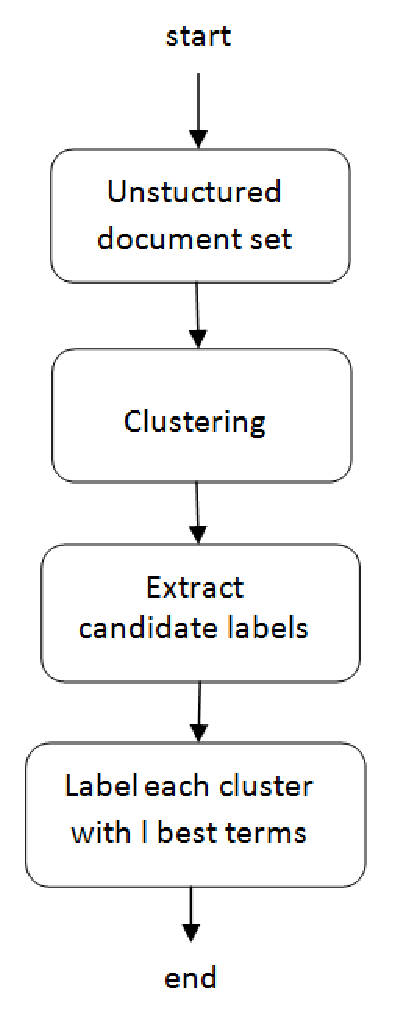
\includegraphics[scale=0.6]{img/wcc}
\caption[Cluster labeling using WCC]%
           {Cluster labeling using Weighted Centroid Covering algorithm}
\label{fig_wcc}
\end{figure}

\gls{WCC} algorithm consists of three stages. As input to the algorithm, a clustering $C$ is given:
\begin{enumerate}
\item For all terms in the input clusters, it saves the $k$ most frequent occurrences of each word with its term frequency, and the cluster in which it occurs, to a data structure (say a vector \L).
\item It sorts vector \text{\L} ~which stores tuples ($k$, $tf(term)$, term, cluster) in a descending order, based on the frequency of a term in a given cluster $tf_{c}(t)$;
\item It assigns $l$ number of terms to each cluster as labels. Therefore, in the end each cluster has a label of $l$ terms, assigned to it in a Round-Robin-like manner. \\
\end{enumerate}

The complexity of \gls{WCC} is $O(\left| T\right . log(\left|T \right|))$. A pseudo code of the algorithm is given as algorithm~\ref{algorithm_wcc}. Additionally, the main steps of \gls{WCC} can be seen graphically in fig.~\ref{fig_wcc}.\\

%\floatname{algorithm}{Procedure}
\renewcommand{\algorithmicrequire}{\textbf{Input:}}
\renewcommand{\algorithmicensure}{\textbf{Output:}}
\begin{algorithm}
\caption{Weighted Centroid Covering algorithm for cluster labeling}
\label{algorithm_wcc}
\begin{algorithmic}
\REQUIRE $C$ - clustering \\
         $l$ - number of terms per label \\
         $k$ - maximum occurrence of the same term in different labels
\ENSURE $\tau$ - labeling function
\STATE $\text{\L} = 0$
\STATE \textbf{foreach} $c$ in $C$ \textbf{do}
\STATE $\tau(c) = 0; $
\STATE \textbf{end foreach}
\STATE \textbf{foreach} $t$ in $T$ \textbf{do}
\FOR{$i = 1$ to $k$}
\STATE compute $c = \kappa(t,i)$ from $C;$
\STATE add tuple $ \langle t, tf_{c}(t)\rangle$ to $\text{\L};$
\ENDFOR
\STATE \textbf{end foreach}
\STATE \textbf{sort} $\text{\L} $ according to descending term frequencies;
\FOR{$labelcount = 1$ to $l$}
\STATE $assigned = 0;$
\STATE $j = 1;$
\WHILE{$assigned < \left|C\right|$ \AND $j \le \left|\text{\L}\right| $}
\STATE let $t_{j} = \langle t, tf_{c} (t)\rangle$ be $j^{th}$ tuple of \text{\L};
\IF{$\left|\tau(c)\right| < labelcount$}
\STATE $\tau(c) = \tau(c) \cup \{t\}$;
\STATE delete $t_{j}$ from $ \text{\L} ;$
\STATE $assigned = assiged + 1;$
\ENDIF
\STATE $j = j + 1;$
\ENDWHILE
\ENDFOR
\STATE \textbf{foreach} $c$ in $C$ \textbf{do}
\STATE \textbf{do} sort $\tau(c)$
\STATE \textbf{end foreach}
\RETURN $\tau;$
\end{algorithmic}
\end{algorithm}



\section{Cluster labeling using external knowledge}
\gls{WCC} was previously presented as an algorithm for cluster labeling. It nominates cluster labels by selecting as candidate labels the terms with highest frequency of occurrence from the corresponding clusters. In order to improve labeling for users, noun phrases may be considered to be used for labels, as they are intuitively understood by humans, and are more descriptive than single terms. In order to improve labeling, an ontology is used as an external knowledge for the cluster labeling algorithm, and candidate labels are nominated from both the ontology and the terms, which occur most frequently in clusters. Thus, if the ontology fails to provide suitable labels, the label candidates proposed by \gls{WCC} are used. \\

In order to present the approach, first a short overview on ontologies is given. In order to gain more detailed insight, refer to the given reference literature, as it is not the topic of this work to investigate into semantic knowledge and ontologies. 

\subsection{Ontology as a source of external knowledge}
Formal models of the world can be used to provide formal semantics, or machine-interpretable meaning to information, stored as documents, web pages, databases. When models are intended to represent a shared conceptualization, such as classification, they are called ontologies~\cite{SemSearch_IRmodels09}. Or if the classical definition from Gruber~\cite{ontology2005} is used: �Ontologies are specifications of the conceptualizations at a semantic level.� \\

Formal ontologies are represented in logical formalism which allows for indexing, querying, and reference purposes over non-ontological datasets, such as documents, databases [23]. An example for a logical formalism is the ontology language \gls{OWL}\footnote{{http://www.w3.org/TR/owl-features/}, accessed December, 2010}. \\

An ontology is characterized by the following tuple (ordered list): \\
\begin{eqnarray}
O = <C, R, I, A>
\end{eqnarray}

In the equation above $C$ is a set of classes which represent the concepts from a given domain. Examples for concepts can be databases, resources, repositories. $R$ is a set of relations, also called properties or predicates. These relations are valid between instances of the classes from $C$. As an example: Resource \textit{isStoredIn} Repository. $I$ is a set of instances, having as elements instances to one or more classes, which can also be linked to other instances or values. For example: \textit{manual2} isStoredIn \textit{onlineRepository1}. And finally, $A$ is a set of axioms, or rules, such as for example (TODO: give a meaningful example for an axiom). \\

According to the formal language used for their creation, ontologies can be divided into \textit{lightweight} and \textit{heavyweight}. Heavyweight ontologies possess highly predictive and restrictive concept definitions; as compared to them, lightweight ontologies allow for more efficient and scalable reasoning [23]. Based on the conceptualization that they describe, the ontologies can be divided further into \textit{upper-level}, which model general knowledge and \textit{domain} ontologies, specific to a certain domain (e.g. the domain of CoreMedia \gls{CMS}).

\subsection{TODO: Weighted Centroid Covering augmented by an ontology}
Stein and Meyer zu Eissen~\cite{Stein04topicidentification} point out that this \gls{WCC} could be extended to use existing ontologies and labels, but they provide no experimental results of any kind. \\

Cluster labeling by using \gls{WCC} has certain limitations. It has been suggested~(\cite{Stein04topicidentification}) to use external knowledge during cluster labeling generation, such as an ontology. Other sources~(\cite{cluster_labeling_wiki_2009}) propose using Wikipedia in order to collect candidate labels for the clusters previously created.\\

- a collection of cluster label candidates can be prepared a priori (an ontology) and
reused with no additional computational cost. \\

- candidate labels can come from a different source - a predefined ontology (to guarantee they are comprehensible). Thus, cluster label comprehensibility and cluster descriptions can be improved by using data extracted from a predefined ontology\\

It is proposed to use external knowledge during the phase extraction of candidate la-
bels (fig.~\ref{fig_wcc_onto}). \\

% wcc with ontology
\begin{figure}
\centering
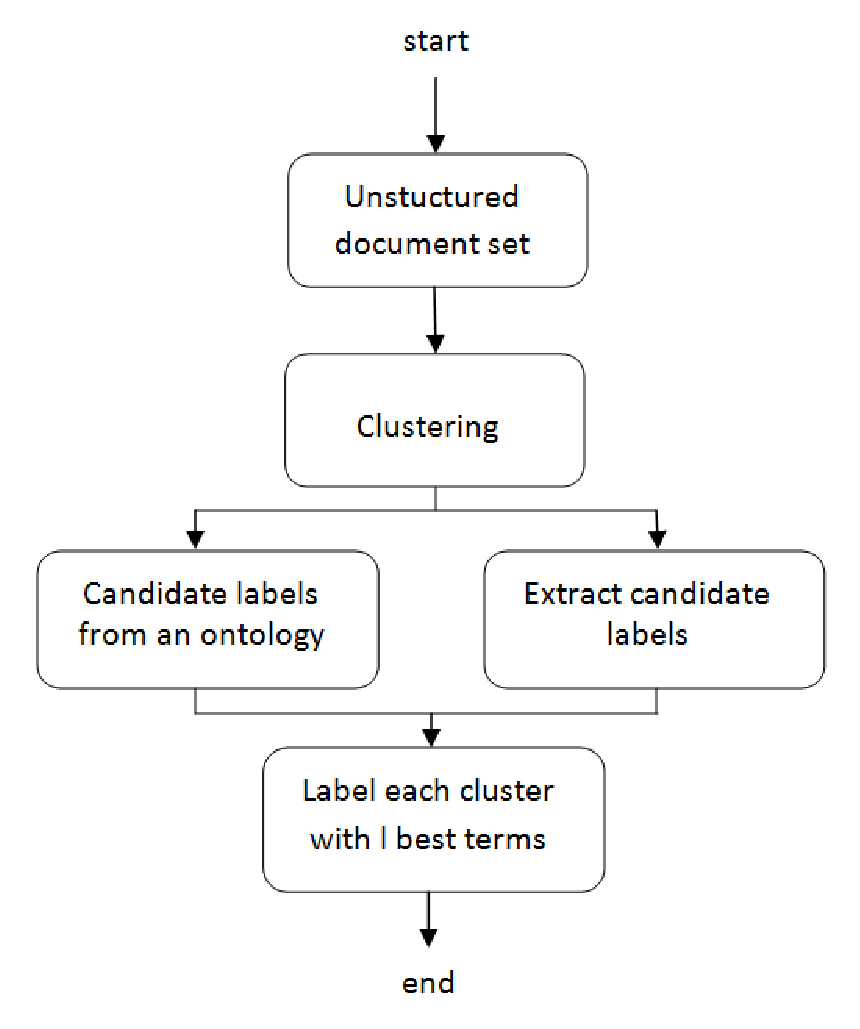
\includegraphics[scale=0.6]{img/wcc-onto}
\caption[Cluster labeling using WCC with external knowledge]%
           {Cluster labeling using Weighted Centroid Covering algorithm, augmented by an ontology}
\label{fig_wcc_onto}
\end{figure}



candidate labels are extracted from an ontology in addition to the important terms that are extracted directly from the cluster content. Thus, selected ontological categories "compete" with inner terms for serving as the cluster labels. In general, prepared ontological categories are a successful resource for labeling; however, inner terms should be considered for the cases when the ontology fails to cover the cluster content. \\

%The best scenario is that cluster labels should present a conceptualization of the documents in text corpus. This is not achieved by the algorithm presented. Technically, a hierarchical clustering algorithm can construct from each Document set $D$ a category tree. However, the labeling based on this hierarchical clustering will be far from a semantical taxonomy. This weakness of the algorithm presented can be corrected by using an external classification knowledge, e.g. an upper-level ontology. \\

%Unfortunately, domain ontologies usually have coverage limitations because not all the terms of the domain are included in the ontology.\\

%Classical clustering methods are not able to deal with the semantics of the linguistic values of the objects (notions, texts). In this paper, a general methodology to incorporate this knowledge into the cluster labeling process has been presented. \\

%We believe that the weaknesses of topic identification algorithms in categorizing search engines could be overcome if external classification knowledge were brought in. We now outline the ideas of such an approach where both topic descriptors and hierarchy information from an upper ontology are utilized. \\

% Then, topic identification is based on the following paradigms:\\
%1. Initially, no hierarchy (refines-relation) is presumed among the C 2 C. This is in accordance with the observations made in [Ert?z et al. 2001].\\
%2. Each category C 2 C is associated to its most similar set O 2 O. If the association is unique, $ T o (O)$ is selected as category label for C.\\
%3. Categories which cannot be associated uniquely within O are treated by a polythetic, equivalence-presuming labeling strategy in a standard way.
%In essence, finding a labeling for a categorization C using an ontology O means to construct a hierarchical classifier, since one has to map the centroid vectors of the clusters C 2 C onto the best-matching O 2 O. Note that a variety of machine learning techniques has successfully been applied to this problem; they include Bayesian classifiers, SVMs, decision trees, neural networks, regression techniques, and nearest neighbor classifiers. \\

Due to time constrains, no experimental results can be provided on running \gls{WCC} with external knowledge. This remains for further work. \\

